    \subsection{発展}\label{節：発展難易度}\label{節：大学過去問ベースのもの}
      ここでは,\bookterm{recurrence}{漸化式}を場合の数,確率,整数,図形,積分,\bookterm{limit}{極限}の問題に使う10題を扱う.
      まず何を\bookterm{sequence}{数列}として追うかを選び,元の条件から\bookterm{recurrence}{漸化式}を立て,最後に元の問いへ戻そう.
      \bookterm{general}{一般項}を求めることだけが目的ではない. 求めたい量の性質に応じて,和,差,剰余,\bookterm{invariant}{不変量}にも注目する.
      問1から問9は大学入試問題の構造・発想を参考に,問いや誘導を本書向けに再構成した演習である.
      問10は著者の掲載問題を改稿したもので,完全順列の古典的題材を扱う.
      参考資料は各問の末尾に示す. 問5は数学IIIの置換積分・部分積分・断面積による体積計算を前提とする.

      \subsubsection{問題}\label{節：発展難易度：問題}\label{節：大学過去問ベースのもの：問題}
        \begin{enumerate}[label=\textbf{問\arabic*.},leftmargin=3.8em,format=\bookitemlink{practice-entrance}{problem}{answer}]
          % F1: 正方形上の確率移動と分布の収束
          \item 正方形の頂点を時計回りに$A,B,C,D$とする.点$P$は初め$A$にあり,1秒ごとに,その頂点にとどまる,時計回りに隣の頂点へ移る,反時計回りに隣の頂点へ移る,の3つの操作から1つを選ぶ.どの操作も選ばれる確率は$\dfrac13$であり,各回の選択は独立である.
                $n$秒後に$P$が$A,C$にいる確率をそれぞれ$p_n,q_n$,\,$B,D$のいずれかにいる確率を$r_n$とする.ただし,\,$n=0,1,2,\ldots$である.

                \smallskip
                \noindent (1)~$p_{n+1},q_{n+1}$を$p_n,q_n,r_n$で表せ.

                \smallskip
                \noindent (2)~$u_n=p_n+q_n$,\,$v_n=p_n-q_n$とおく.$u_n,v_n$の\bookterm{general}{一般項}を求め,各頂点にいる確率を求めよ.

                \smallskip
                \noindent (3)~各頂点にいる確率の$n\to\infty$における\bookterm{limit}{極限}を求めよ.
                \par\smallskip{\small\textit{\href{https://www.u-tokyo.ac.jp/content/400263415.pdf}{東京大学2024年理科第3問の状態分類を参考に再構成}}}
          % F2: 奇数が続く条件と2の因子
          \item 正の整数$a_0$から,\bookterm{sequence}{数列}$\{a_n\}$を
                \[
                  a_{n+1}=\begin{cases}
                    \dfrac{a_n}{2}&(a_n\text{が偶数}),\\[3pt]
                    \dfrac{3a_n+1}{2}&(a_n\text{が奇数})
                  \end{cases}
                \]
                によって定める.

                \smallskip
                \noindent (1)~$a_0,a_1,\ldots,a_m$がすべて奇数であるとき,$a_j+1$を$a_0$と$j$で表せ.ただし,\,$0\le j\le m$とする.

                \smallskip
                \noindent (2)~正整数$m$に対し,$a_0,a_1,\ldots,a_m$がすべて奇数となるような$a_0$をすべて求め,その最小値を答えよ.

                \smallskip
                \noindent (3)~$a_0+1=2^s t$と表す.ただし,\,$s$は$0$以上の整数,$t$は正の奇数である.初項$a_0$から連続して現れる奇数項の個数を求めよ.
                \par\smallskip{\small\textit{\href{https://www.kyoto-u.ac.jp/ja/admissions/undergrad/past-eq}{京都大学2024年理系第4問の偶奇分岐を参考に再構成}}}
          % F3: 畳み込み和が一定になる数列
          \item \bookterm{sequence}{数列}$\{c_n\}$を
\BookMathLayout{\[
                  c_0=1,\qquad
                  c_{n+1}=\frac{2n+1}{2n+2}c_n
                  \quad(n=0,1,2,\ldots)
                \]}{
\[
\begin{aligned}
c_0&=1,\\
c_{n+1}&=\frac{2n+1}{2n+2}c_n\\
&\quad(n=0,1,2,\ldots)
\end{aligned}
\]
}
                によって定め,
                \[
                  T_n=\sum_{k=0}^{n}c_kc_{n-k}
                \]
                とする.

                \smallskip
                \noindent (1)~$c_n$を階乗を用いて表せ.ただし,\,$0!=1$とする.

                \smallskip
                \noindent (2)~正整数$n$に対し,
                \[
                  nT_n=\sum_{j=0}^{n-1}(2j+1)c_jc_{n-1-j}
                \]
                を示せ.さらに,この等式を用いて$T_n$を求めよ.

                \smallskip
                \noindent (3)~正整数$n$に対し,
                \[
                  \sum_{k=0}^{n}\binom{2k}{k}
                     \binom{2n-2k}{n-k}=4^n
                \]
                が成り立つことを示せ.
                \par\smallskip{\small\textit{\href{https://www.osaka-u.ac.jp/ja/admissions/faculty/general/files/9o1vy3/@@download/file}{大阪大学2025年文系第2問の\bookterm{convolution}{畳み込み}構造を参考に再構成}}}
          % F4: 内分を繰り返す平行四辺形
          \item 平行四辺形$A_0B_0C_0D_0$の頂点を反時計回りに並べる.
                一定の実数$t$が$0<t<1$を満たすとする.
                四角形$A_nB_nC_nD_n$の各辺上に,
                \[
                 \begin{aligned}
                 A_nA_{n+1}:A_{n+1}B_n&=t:(1-t),\\
                 B_nB_{n+1}:B_{n+1}C_n&=t:(1-t),\\
                 C_nC_{n+1}:C_{n+1}D_n&=t:(1-t),\\
                 D_nD_{n+1}:D_{n+1}A_n&=t:(1-t)
                 \end{aligned}
                \]
                となる点を取り,この操作を繰り返す.\,$n$は$0$以上の整数とする.
                \par\noindent
                (1) 各四角形は平行四辺形であり,対角線の交点が変わらないことを示せ.
                \par\noindent
                (2) $A_nB_nC_nD_n$の面積を$S_n$とする.\,$S_n$を$S_0,t,n$で表せ.
                \par\noindent
                (3) $n\to\infty$のとき,すべての頂点が最初の対角線の交点$O$に近づくことを示せ.
                \par\noindent
                (4) 初めの図形が辺長$\ell$の正方形で,\,$\displaystyle t=\frac{1}{2}$の場合を考える.
                操作を$n$回行った正方形の辺長を求めよ.
                また,有向線分$A_nB_n$の向きは,最初の向きからどれだけ回転するか.
                \par\smallskip{\small\textit{\href{https://www.densu.jp/tsukuba/22tsukubaspass.pdf}{筑波大学2022前期 第3問の内分操作を参考に独自に再構成}}}
          % F5: 積分を数列にして円錐を切る
          \item この問題では,数学IIIの部分積分・置換積分と,断面積による体積計算を用いる.
                正整数$n$に対して,
                \[
                 I_n=\int_0^{\frac{\pi}{3}}\frac{d\theta}{\cos^n\theta}
                \]
                とする.
                \par\noindent
                (1) $I_1,I_2$を求めよ.
                \par\noindent
                (2) $n\geq3$について$\,I_n$と$I_{n-2}$の関係式を求め,\,$I_3$を計算せよ.
                \par\noindent
                (3) 座標空間において,原点を頂点とし,平面$z=2$上の半径$2$の円を底面とする円錐を考える.
                その内部と表面は,
                \[
                 0\leq z\leq2,\qquad x^2+y^2\leq z^2
                \]
                で表される.この円錐のうち$x\geq1$を満たす部分の体積を求めよ.
                \par\smallskip{\small\textit{\href{https://www.nagoya-u.ac.jp/admissions/exam/upload/06_h31_sugakurikakei-seikai.pdf}{名古屋大学2019理系 第1問の構造を参考に独自に再構成}}}
          % F6: 一般項を求めずに減衰の速さを決める
          \item $\displaystyle a_1=1,\qquad
                a_{n+1}=\frac{a_n}{(1+2a_n)^2}$
                で\bookterm{sequence}{数列}$\{a_n\}$を定め,$\displaystyle b_n=\frac{1}{a_n}$とする.
                \par\noindent
                (1) すべての項が正であることを確かめ,$n\geq2$について$b_n>4n-3$を示せ.
                \par\noindent
                (2) 次の\bookterm{limit}{極限}を求めよ.
                \[
                 \lim_{n\to\infty}\frac1n\sum_{k=1}^n a_k
                \]
                (3) $\displaystyle\lim_{n\to\infty}na_n$を求めよ.
                \par\smallskip{\small\textit{\href{https://toudainyuushi.com/wp-content/uploads/2020/06/2006S.pdf}{東京大学2006理科 第5問を参考に再構成した既存題を維持・増補}}}
          % F7: 1往復で整列できる札の配置
          \item $n$枚の札には$1,2,\ldots,n$の数字が1つずつ書かれている.
                これらを横一列に並べ, 隣り合う2枚を左から順に調べる.
                左の数字が右の数字より大きいときだけ交換し, 右端まで進む.
                続いて, 隣り合う2枚を右から順に調べ, 同じ規則で交換して左端まで戻る.
                この1往復で$1,2,\ldots,n$の順になる初期配置を\textbf{成功配置}と呼び, その個数を$c_n$とする.
                ただし,\,$n=1$では操作を行わず,\,$c_1=1$とする. 以下の問に答えよ.

                \smallskip
                \noindent (1)~$c_2,c_3$を求めよ. また,\,$n\ge2$として成功配置の最初の2枚の数字を$A_1,A_2$とするとき,
                少なくとも一方が$2$以下であることを示せ.

                \smallskip
                \noindent (2)~$n\ge3$とする. 最初の2枚に$1$を含む場合と,\,$1$を含まず$2$を含む場合に分けて数え,
                $c_n,c_{n-1},c_{n-2}$の関係式を求めよ.
                後者では, 最初の比較を済ませてから$2$の札を取り除くことを考えてよい.

                \smallskip
                \noindent (3)~$c_n$を求めよ.
                \par\smallskip{\small\textit{\href{https://www.u-tokyo.ac.jp/content/400239118.pdf}{東京大学2025年度理科第5問を参考に再構成}}}
          % F8: 巨大な項の整除と, 添字の互除法
          \item $\displaystyle a_1=1,\quad a_{n+1}=a_n^2+1$
                で定まる\bookterm{sequence}{数列}$\{a_n\}$について, 以下の問に答えよ.
                整数$x,y$の最大公約数を$\gcd(x,y)$と表す.

                \smallskip
                \noindent (1)~$a_n$が$5$の倍数となる正整数$n$をすべて求めよ.

                \smallskip
                \noindent (2)~任意の正整数$m,n$に対して,\,$a_m$が$a_n$を割り切ることと,
                $m$が$n$を割り切ることは同値であることを示せ.
                必要なら, 補助的に$a_0=0$と定めてよい.

                \smallskip
                \noindent (3)~任意の正整数$m,n$について
                \[
                 \gcd(a_m,a_n)=a_{\gcd(m,n)}
                \]
                が成り立つことを示し,\,$\gcd(a_{2026},a_{3040})$を求めよ.
                \par\smallskip{\small\textit{\href{https://www.densu.jp/tokyo/22tokyospass.pdf}{東京大学2022年度理科第2問を参考に再構成}}}
          % F9: 整数方程式の解を生み出す漸化式
          \item 正の整数$x,y,z$についての方程式
                \[
                 x^2+y^2+z^2=xyz
                \]
                を考える. 以下の問に答えよ.

                \smallskip
                \noindent (1)~$x=3$を満たす解$(3,y,z)$について,\,$y\le z$ならば
                $(3,z,3z-y)$も正の整数解であり,\,$3z-y>z$となることを示せ.

                \smallskip
                \noindent (2)~\bookterm{sequence}{数列}$\{u_n\}$を
                \[
                 u_0=u_1=3,\qquad
                 u_{n+2}=3u_{n+1}-u_n\quad(n\ge0)
                \]
                によって定める. \bookterm{general}{一般項}を求めよ.

                \smallskip
                \noindent (3)~$(3,u_n,u_{n+1})$がすべての$n\ge0$について上の方程式の正の整数解となることを示せ.
                さらに, 異なる正の整数解が無限個あることを示し,
                $\displaystyle\lim_{n\to\infty}\frac{u_{n+1}}{u_n}$を求めよ.
                \par\smallskip{\small\textit{\href{https://toudainyuushi.com/wp-content/uploads/2020/06/2006S.pdf}{東京大学2006年度理科第4問を参考に独自に作成}}}
          % F10: 元のペアをすべて解消する組み替え
          \item $n$を正の整数とする. 互いに異なる$2n$個の要素
                \[
                 A_1,\ldots,A_n,\quad B_1,\ldots,B_n
                \]
                があり, 初めは$A_i$と$B_i$がペアを組んでいる.
                各ペアを$A$側と$B$側から1個ずつ選んで作り, すべての要素をちょうど1回ずつ使って$n$組のペアを作り直す.
                完成した組合せを数え, ペアを並べる順序や組み替える操作の手順は区別しない.
                元のペア$(A_i,B_i)$が1組も残らない組合せの数を$S(n)$とする.
                以下,\,$S(0)=1$と定める.
                \par\smallskip
                (1) $S(1),S(2),S(3)$を求めよ.
                \par\smallskip
                (2) $A_1$の相手を$B_j$とする.
                $A_j$の相手が$B_1$である場合と, そうでない場合に分け,
                $S(n),S(n-1),S(n-2)$の関係式を求めよ.
                \par\smallskip
                (3) $S(n)-nS(n-1)$を求め,\,$S(n)$を有限和で表せ.
                \par\smallskip
                (4) $r$を$0\le r\le n$を満たす整数とする.
                元のペアがちょうど$r$組残る組合せの数を求めよ.
                また, 全$n!$通りの組合せについて, 元のペアが残る組数の平均値を求めよ.
                \par\smallskip{\small\textit{\href{https://jukenmath.net/problems/798}{著者作問「ペアの入れ替えパターン数」}}}
        \end{enumerate}

      \subsubsection{方針}\label{節：発展難易度：方針}\label{節：大学過去問ベースのもの：方針}
        \begin{enumerate}[label=\textbf{問\arabic*.},leftmargin=3.8em,format=\bookitemlink{practice-entrance}{hint}{problem}]
          % F1: 正方形上の確率移動と分布の収束
          \item $A$への移動は,$A$にとどまる場合と,$B,D$から移る場合に分かれる.$p_n+q_n+r_n=1$を使って和の式から$r_n$を消去する.差の式では$r_n$が相殺する.$B,D$にいる確率が等しいことも,操作の対称性から確かめる.
          % F2: 奇数が続く条件と2の因子
          \item 奇数の分岐だけを使える間は,$a_{n+1}+1=\dfrac32(a_n+1)$となる.(2)では,$a_m+1$が偶数になる必要条件を求めた後,その条件から実際に各項が奇数になることを確認する.(3)では,$a_j+1$から2の因子が1つずつ減ることに注目する.
          % F3: 畳み込み和が一定になる数列
          \item (1)は\bookterm{ratio}{階比}型として係数を掛ける.(2)では,$n=k+(n-k)$と分け,\,$k$を$n-k$に入れ替えて同じ和が現れることを使う.\bookterm{recurrence}{漸化式}で$kc_k$を$c_{k-1}$に直した後も,添字を逆順にした2つの式を加えると係数が一定になる.(3)は(1)の式を$T_n$に代入する.
          % F4: 内分を繰り返す平行四辺形
          \item 隣接する辺を$\boldsymbol p_n=\overrightarrow{A_nB_n}$,
                \,$\boldsymbol q_n=\overrightarrow{A_nD_n}$とする.
                面積は,内側の四角形の周囲に残る四つの三角形を引けばよい.
                収束を示すときは,\,$|\boldsymbol p_n|^2+|\boldsymbol q_n|^2$の\bookterm{recurrence}{漸化式}を作る.
                正方形の場合は,辺を表す複素数への掛け算で回転を読み取る.
          % F5: 積分を数列にして円錐を切る
          \item $I_n$を$\cos^{-(n-2)}\theta$と$\cos^{-2}\theta$の積として部分積分し,
                $\sin^2\theta=1-\cos^2\theta$で整理する.
                体積は平面$z=$一定で切る.断面は半径$z$の円の弓形になるので,
                弓形の半分の中心角を$\theta$とし,$z\cos\theta=1$で置換する.
          % F6: 一般項を求めずに減衰の速さを決める
          \item 逆数を取ると,$b_{n+1}-b_n=4+4a_n$になる.
                \bookterm{difference}{階差}を足し合わせた式を使い,まず$a_n\to0$を示す.
                平均の\bookterm{limit}{極限}は,有限個の初期項と,十分小さくなった残りの項に分けて評価する.
                最後に$\displaystyle \frac{b_n}{n}$を調べ,$na_n$へ戻す.
          % F7: 1往復で整列できる札の配置
          \item 最初の比較の後, 左端には$\min(A_1,A_2)$が残る. この札がその後で触れられるのは, 復路の最後の比較だけである.
                個数を数える際には, 最初の2枚のどちらに$1$または$2$があるかで4つに分ける.
                $1$を取り除く場合と$2$を取り除く場合は, 小さい配置との対応が異なることに注意する.
          % F8: 巨大な項の整除と, 添字の互除法
          \item (1)では項そのものを計算する代わりに,\,$5$で割った余りに\bookterm{recurrence}{漸化式}を適用する.
                (2)では法を$a_m$へ変える. $a_0=0$とおけば,\,$a_m$から先の余りは$a_0$からの余りを繰り返す.
                (3)では$n$を$m$で割った余りへ置き換える操作が, 項の最大公約数を変えないことを示す.
          % F9: 整数方程式の解を生み出す漸化式
          \item (1)では$9+z^2+(3z-y)^2-3z(3z-y)$を整理する.
                この整理で保たれる式を,\,(3)では隣接する2項に適用する.
                (2)は実数解型の3項間\bookterm{recurrence}{漸化式}である. (3)の整数性は\bookterm{general}{一般項}を展開するよりも, 初期値と\bookterm{recurrence}{漸化式}から示す方が短い.
          % F10: 元のペアをすべて解消する組み替え
          \item (2) 後者では,\,$B_1$の相手を$A_k$とする.
                $A_1,B_1$を除き,\,$A_k$と$B_j$をペアにして,\,$n-1$組の問題との対応を考える.
                (3) 3項間の関係式を,\,$S(n)-nS(n-1)$について書き直す.
                その後,\,$n!$で割って\bookterm{difference}{階差}を作る.
                (4) 残すペアを選んでから, 残りを完全に組み替える.
                平均値は, 各元のペアが何通りの組合せに含まれるかを数えると短い.
        \end{enumerate}

      \subsubsection{答え}\label{節：発展難易度：解答}\label{節：大学過去問ベースのもの：解答}
        \begin{enumerate}[label=\textbf{問\arabic*.},leftmargin=3.8em,format=\bookitemlink{practice-entrance}{answer}{problem}]
          % F1: 正方形上の確率移動と分布の収束
          \item (1)~
                \[
                  p_{n+1}=\frac{p_n+r_n}{3},\qquad
                  q_{n+1}=\frac{q_n+r_n}{3}.
                \]
                (2)~
                \[
                \begin{aligned}
                  u_n&=\frac12+\frac12\left(-\frac13\right)^n,\\
                  v_n&=\left(\frac13\right)^n.
                \end{aligned}
                \]
                したがって
                \[
                \begin{aligned}
                  p_n&=\frac14+\frac12\left(\frac13\right)^n
                       +\frac14\left(-\frac13\right)^n,\\
                  q_n&=\frac14-\frac12\left(\frac13\right)^n
                       +\frac14\left(-\frac13\right)^n.
                \end{aligned}
                \]
                $B,D$にいる確率はそれぞれ
                \[
                  \frac14-\frac14\left(-\frac13\right)^n
                \]
                である.(3)~\bookterm{limit}{極限}はいずれも$\dfrac14$である.
          % F2: 奇数が続く条件と2の因子
          \item (1)~
                \[
                  a_j+1=\frac{3^j}{2^j}(a_0+1)
                  \quad(0\le j\le m).
                \]
                (2)~求める初期値は
                \[
                  a_0=2^{m+1}\ell-1
                  \quad(\ell=1,2,3,\ldots)
                \]
                であり,最小値は$2^{m+1}-1$である.

                (3)~奇数項の個数は$s$である.$s\ge1$のとき,$a_0,\ldots,a_{s-1}$が奇数であり,$a_s=3^s t-1$は偶数である.$s=0$のときは初項から偶数である.
          % F3: 畳み込み和が一定になる数列
          \item (1)~
                \[
                  c_n=\frac{(2n)!}{4^n(n!)^2}
                     =\frac1{4^n}\binom{2n}{n}.
                \]
                (2)~設問の等式から$T_n=T_{n-1}$が得られ,$T_0=1$より
                \[
                  T_n=1\quad(n=0,1,2,\ldots).
                \]
                (3)~$c_kc_{n-k}$を(1)の式で表し,$T_n=1$の両辺を$4^n$倍すれば示される.
          % F4: 内分を繰り返す平行四辺形
          \item (1) 対角線の交点は常に$O$である.
                \par\noindent
                (2) $\rho=(1-t)^2+t^2$と置くと,
                \[
                 S_n=S_0\rho^n.
                \]
                (3) 四つの頂点はすべて$O$に近づく.
                \par\noindent
                (4) 辺長は$\ell\,2^{-\frac{n}{2}}$であり,有向線分の向きは反時計回りに$\displaystyle \frac{n\pi}{4}$だけ回転する.
                向きの角は$2\pi$の整数倍の違いを同一視する.
          % F5: 積分を数列にして円錐を切る
          \item (1)
                \[
                 I_1=\log(2+\sqrt3),\qquad I_2=\sqrt3.
                \]
                (2)
                \[
                 (n-1)I_n=(n-2)I_{n-2}+2^{n-2}\sqrt3,
                \]
                \[
                 I_3=\sqrt3+\frac12\log(2+\sqrt3).
                \]
                (3) 求める体積は
                \[
                 \frac{8\pi}{9}-\frac{4\sqrt3}{3}
                 +\frac13\log(2+\sqrt3).
                \]
                ここで$\log$は自然\bookterm{logarithm}{対数}である.
          % F6: 一般項を求めずに減衰の速さを決める
          \item (1) すべての項は正であり,
                \[
                 b_n=4n-3+4\sum_{k=1}^{n-1}a_k>4n-3
                 \qquad(n\geq2).
                \]
                (2) \bookterm{limit}{極限}は$0$である.
                \par\noindent
                (3) \bookterm{limit}{極限}は$\displaystyle \frac{1}{4}$である.
          % F7: 1往復で整列できる札の配置
          \item (1)~$c_2=2,\ c_3=6$である.

                (2)~$n\ge3$に対して
                \[
                  c_n=4c_{n-1}-2c_{n-2}.
                \]
                (3)~したがって,
                \[
                  \boxed{\displaystyle
                  c_n=\frac{(2+\sqrt2)^{n-1}+(2-\sqrt2)^{n-1}}2}
                  \quad(n\ge1).
                \]
          % F8: 巨大な項の整除と, 添字の互除法
          \item (1)~$n=3,6,9,\ldots$, すなわち$3$の正の倍数である.

                (2)~$a_m\mid a_n\ \Longleftrightarrow\ m\mid n$である.

                (3)~$\gcd(a_m,a_n)=a_{\gcd(m,n)}$であり,
                \[
                 \boxed{\gcd(a_{2026},a_{3040})=a_2=2}.
                \]
          % F9: 整数方程式の解を生み出す漸化式
          \item $\displaystyle\alpha=\frac{3+\sqrt5}2,\quad
                \beta=\frac{3-\sqrt5}2$とおくと,
                \[
                 \boxed{\displaystyle
                 u_n=\frac32\left\{
                 \alpha^n+\beta^n-
                 \frac{\alpha^n-\beta^n}{\sqrt5}
                 \right\}}.
                \]
                $(3,u_n,u_{n+1})$は正の整数解であり,\,$n\ge1$で$u_{n+1}>u_n$だから異なる解が無限個得られる.
                また,
                \[
                 \boxed{\displaystyle
                 \lim_{n\to\infty}\frac{u_{n+1}}{u_n}
                 =\frac{3+\sqrt5}2}.
                \]
          % F10: 元のペアをすべて解消する組み替え
          \item (1)
                \[
                 S(1)=0,\quad S(2)=1,\quad S(3)=2.
                \]
                (2)
                \[
                 S(n)=(n-1)\{S(n-1)+S(n-2)\}
                 \quad(n\ge2).
                \]
                (3)
                \[
                 S(n)-nS(n-1)=(-1)^n,
                \]
                \[
                 \boxed{S(n)=n!\sum_{k=0}^{n}\frac{(-1)^k}{k!}}.
                \]
                (4) 組合せの数は
                \[
                 \binom{n}{r}S(n-r).
                \]
                元のペアが残る組数の平均値は$1$である.
        \end{enumerate}

      \subsubsection{解説}\label{節：発展難易度：解法}\label{節：大学過去問ベースのもの：解法}
        \begin{enumerate}[label=\textbf{問\arabic*.},leftmargin=3.8em,format=\bookitemlink{practice-entrance}{solution}{problem}]
          % F1: 正方形上の確率移動と分布の収束
          \item \textbf{(1)~直前の位置で分ける.}
                  $A$にとどまる場合と,$B,D$から移る場合は重ならない.
                  どちらの頂点からも$A$への移動確率は$\dfrac{1}{3}$なので,確率$r_n$にまとめてよい.
                  $C$についても同様であり,
                  \[
                    p_{n+1}=\frac{p_n+r_n}3,\quad q_{n+1}=\frac{q_n+r_n}3.
                  \]
                  \smallskip\textbf{(2)~和と差で解く.}
                  $p_0=1,q_0=r_0=0$と$p_n+q_n+r_n=1$から,和と差は
                  \[
                    u_{n+1}=\frac23-\frac13u_n,\quad u_0=1,
                  \]
                  \[
                    v_{n+1}=\frac13v_n,\quad v_0=1
                  \]
                  を満たす.和では\bookterm{fixed}{不動点}$\dfrac{1}{2}$を引くと,
                  \[
                    u_n=\frac12+\frac12\left(-\frac13\right)^n,\quad
                    v_n=\left(\frac13\right)^n.
                  \]
                  $p_n=\dfrac{u_n+v_n}{2}$, $q_n=\dfrac{u_n-v_n}{2}$で戻す.
                  時計回りと反時計回りを交換する経路の一対一対応は,$A,C$を固定して$B,D$を入れ替え,確率を保つ.
                  よって$B,D$にいる確率はそれぞれ$\dfrac{r_n}{2}=\dfrac{1-u_n}{2}$である.
                  \smallskip\textbf{(3)~出発点の影響が消える.}
                  二つの公比の絶対値は$\dfrac{1}{3}<1$なので,各頂点の確率は$\dfrac{1}{4}$へ近づく.
                  初めの$A$への偏りが消え,対頂点の組$\{A,C\}$にいる確率$u_n$は$\dfrac{1}{2}$の上下を交互に行き来する.
          % F2: 奇数が続く条件と2の因子
          \item \textbf{(1)~分岐を固定する.}
                  奇数が続く区間に限れば$a_{j+1}=\dfrac{3a_j}{2}+\dfrac{1}{2}$である.
                  \bookterm{fixed}{不動点}$-1$を引くと$a_{j+1}+1=\dfrac{3(a_j+1)}{2}$だから,
                  \[
                    a_j+1=\frac{3^j}{2^j}(a_0+1)\quad(0\le j\le m).
                  \]
                  この式を使えるのは,奇数の分岐が続く範囲である.
                  \smallskip\textbf{(2)~必要条件と十分性.}
                  全項$a_0,\ldots,a_m$が奇数なら,
                  \[
                    3^m(a_0+1)=2^m(a_m+1)
                  \]
                  の右辺は$2^{m+1}$で割り切れる.$3^m$と互いに素なので,
                  $a_0=2^{m+1}\ell-1$（$\ell$は正整数）が必要である.
                  逆にこの初項から,
                  \[
                    b_j=3^j2^{m+1-j}\ell-1\quad(0\le j\le m)
                  \]
                  とおくと,すべて正の奇数で,$b_0=a_0$かつ$\dfrac{3b_j+1}{2}=b_{j+1}$（$0\le j<m$）である.
                  実際に奇数の分岐で進むため$a_j=b_j$となり,十分性も示せた.
                  最小値は$\ell=1$の$2^{m+1}-1$である.
                  \smallskip\textbf{(3)~奇数区間の長さ.}
                  $s=0$なら初項が偶数なので答えは$0$である.
                  $s\ge1$なら,同じ確認から
                  \[
                    a_j=3^j2^{s-j}t-1\quad(0\le j\le s)
                  \]
                  となる.$j<s$では奇数,$j=s$では偶数なので連続する奇数項は$s$個である.
                  例えば$a_0=7$では$7,11,17,26,\ldots$となる.
                  最初の奇数区間の長さは,$a_0+1$に含まれる$2$の因子で決まる.
          % F3: 畳み込み和が一定になる数列
          \item \textbf{(1)~\bookterm{ratio}{階比}型で各項を求める.}
                  偶数の積は$2^nn!$,奇数の積は$\dfrac{(2n)!}{2^nn!}$なので,
                  \[
                    c_n=\prod_{j=0}^{n-1}\frac{2j+1}{2j+2}
                       =\frac{(2n)!}{4^n(n!)^2}.
                  \]
                  $n=0$では空積を$1$とする.
                  \smallskip\textbf{(2)~和そのものを追う.}
                  階乗の式を直接代入する代わりに,$T_n$の更新を探す.
                  $n=k+(n-k)$を掛け,第2の和の添字を逆順にすると,
                  \[
                  \begin{aligned}
                    nT_n&=\sum_{k=0}^n kc_kc_{n-k}
                          +\sum_{k=0}^n(n-k)c_kc_{n-k}\\
                        &=2\sum_{k=1}^n kc_kc_{n-k}.
                  \end{aligned}
                  \]
                  $k=0$の項は零である.$2kc_k=(2k-1)c_{k-1}$と$j=k-1$から,
                  \[
                    nT_n=\sum_{j=0}^{n-1}(2j+1)c_jc_{n-1-j}=U_n.
                  \]
                  今度は$j$を$n-1-j$に入れ替えると,
                  \[
                    U_n=\sum_{j=0}^{n-1}(2n-2j-1)c_jc_{n-1-j}.
                  \]
                  二式を加えると係数が$2n$でそろうため,$2U_n=2nT_{n-1}$となる.
                  $n\ge1$で割れば$T_n=T_{n-1}$であり,$T_0=1$から$T_n=1$を得る.
                  添字の和が一定で,二つの添字を交換しても積が変わらないことが決め手だった.
                  \smallskip\textbf{(3)~二項係数の恒等式.}
                  (1)から,
                  \[
                    c_kc_{n-k}=\frac1{4^n}\binom{2k}{k}
                                              \binom{2n-2k}{n-k}.
                  \]
                  $T_n=1$を$4^n$倍すれば設問の恒等式となる.
                  例えば$n=2$では$1\cdot6+2\cdot2+6\cdot1=16$である.
                  複雑な各項でも,和を一つの\bookterm{sequence}{数列}として追うと簡単な性質が現れる.
          % F4: 内分を繰り返す平行四辺形
          \item 図形が変わるたびに四つの頂点を別々に追うと,計算が増える.
                平行四辺形を決める二本の辺と,図形の中心に注目する.
                \par\noindent
                \textbf{(1) 内分をベクトルで表す.}
                位置ベクトルを$\boldsymbol a_n,\boldsymbol b_n,
                \boldsymbol c_n,\boldsymbol d_n$とする.
                内分の条件より,
                \[
                 \begin{aligned}
                 \boldsymbol a_{n+1}&=(1-t)\boldsymbol a_n+t\boldsymbol b_n,\\
                 \boldsymbol b_{n+1}&=(1-t)\boldsymbol b_n+t\boldsymbol c_n,\\
                 \boldsymbol c_{n+1}&=(1-t)\boldsymbol c_n+t\boldsymbol d_n,\\
                 \boldsymbol d_{n+1}&=(1-t)\boldsymbol d_n+t\boldsymbol a_n.
                 \end{aligned}
                \]
                いま,$A_nB_nC_nD_n$が平行四辺形で,中心の位置ベクトルが$\boldsymbol o$なら,
                \[
                 \boldsymbol a_n+\boldsymbol c_n
                 =\boldsymbol b_n+\boldsymbol d_n=2\boldsymbol o.
                \]
                したがって,
                \[
                 \begin{aligned}
                 \boldsymbol a_{n+1}+\boldsymbol c_{n+1}
                  &=(1-t)\,2\boldsymbol o+t\,2\boldsymbol o\\
                  &=2\boldsymbol o,
                 \end{aligned}
                \]
                同様に$\boldsymbol b_{n+1}+\boldsymbol d_{n+1}=2\boldsymbol o$である.
                二本の対角線は同じ点$O$で二等分されるので,次の図形も平行四辺形で,中心は変わらない.
                初めの図形は平行四辺形だから,この性質は\bookterm{induction}{数学的帰納法}ですべての$n$について成り立つ.
                \par\noindent
                \textbf{(2) 面積を\bookterm{sequence}{数列}にする.}
                内側の四角形の周囲には四つの三角形が残る.
                たとえば頂点$A_n$にある三角形$A_nA_{n+1}D_{n+1}$では,
                二辺がそれぞれ$|A_nB_n|$の$t$倍と$|A_nD_n|$の$1-t$倍である.
                よって面積は$\frac12t(1-t)S_n$になる.
                ほかの三つも同じ面積なので,
                \[
                 \begin{aligned}
                 S_{n+1}
                 &=S_n-4\cdot\frac12t(1-t)S_n\\
                 &=\{(1-t)^2+t^2\}S_n.
                 \end{aligned}
                \]
                ここで初めて,図形の問いが本編の等比型になった.
                \,$\rho=(1-t)^2+t^2$と置けば,
                \[
                 S_n=S_0\rho^n.
                \]
                $\rho>0$なので面積は常に正であり,各平行四辺形は退化しない.
                \par\noindent
                \textbf{(3) 頂点の収束を調べる.}
                面積が$0$に近づくだけでは,細長い図形になる可能性を除けない.
                そこで,二本の辺の長さも調べる.
                \[
                 \boldsymbol p_n=\boldsymbol b_n-\boldsymbol a_n,
                 \qquad
                 \boldsymbol q_n=\boldsymbol d_n-\boldsymbol a_n
                \]
                とすると,内分の式と平行四辺形の性質より,
                \[
                 \begin{cases}
                 \boldsymbol p_{n+1}=(1-t)\boldsymbol p_n+t\boldsymbol q_n,\\
                 \boldsymbol q_{n+1}=-t\boldsymbol p_n+(1-t)\boldsymbol q_n.
                 \end{cases}
                \]
                連立式から一つの\bookterm{sequence}{数列}を取り出すため,長さの二乗を足した
                \[
                 E_n=|\boldsymbol p_n|^2+|\boldsymbol q_n|^2
                \]
                を考える.内積の交差項が打ち消し合うので,
                \[
                 \begin{aligned}
                 E_{n+1}
                 &=|(1-t)\boldsymbol p_n+t\boldsymbol q_n|^2\\
                 &\quad+|-t\boldsymbol p_n+(1-t)\boldsymbol q_n|^2\\
                 &=\rho E_n.
                 \end{aligned}
                \]
                よって$E_n=\rho^nE_0$である.
                $0<t<1$より$0<\rho=1-2t(1-t)<1$である.
                二乗は非負だから,両方の辺の長さは$0$へ近づく.
                また,$O$は対角線の中点なので,
                \[
                 \overrightarrow{OA_n}=-\frac{\boldsymbol p_n+\boldsymbol q_n}{2},
                 \qquad
                 |OA_n|\leq\frac{|\boldsymbol p_n|+|\boldsymbol q_n|}{2}.
                \]
                右辺は$0$に近づく.ほかの頂点についても$\boldsymbol p_n,\boldsymbol q_n$の符号が変わるだけだから,
                同じ評価ができる.したがって四つの頂点はすべて$O$に近づく.
                \par\noindent
                \textbf{(4) 正方形と複素数の積.}
                正方形が反時計回りに並んでいるとき,$\boldsymbol q_n$は$\boldsymbol p_n$を反時計回りに$\displaystyle \frac{\pi}{2}$回転したものである.
                それぞれを表す複素数を$z_n,w_n$とすると,$w_n=iz_n$である.
                \,$\displaystyle t=\frac{1}{2}$を連立式に入れると,
                \[
                 z_{n+1}=\frac{1+i}{2}z_n,
                 \qquad
                 w_{n+1}=iz_{n+1}.
                \]
                したがって次も正方形であり,
                \[
                 z_n=\left(\frac{1+i}{2}\right)^n z_0.
                \]
                ここで,
                \[
                 \frac{1+i}{2}
                 =\frac1{\sqrt2}\left(\cos\frac\pi4+i\sin\frac\pi4\right).
                \]
                \bookterm{de-moivre}{ド・モアブルの定理}より,
                \[
                 z_n=2^{-\frac{n}{2}}
                 \left(\cos\frac{n\pi}{4}+i\sin\frac{n\pi}{4}\right)z_0.
                \]
                よって辺長は$\ell\,2^{-\frac{n}{2}}$,有向線分の回転角は反時計回りに$\displaystyle \frac{n\pi}{4}$である.
                \par
                正方形では内分という操作が,中心を固定した回転と縮小そのものになる.
                一般の平行四辺形については,二本の辺を混ぜる連立式と面積の等比性が成り立つが,
                図形全体が毎回同じ平面回転と一様な縮小を受けるとは限らない.
          % F5: 積分を数列にして円錐を切る
          \item ここでは\bookterm{sequence}{数列}の項が積分で定義されている.
                各積分を別々に計算するのでなく,べきの指数が異なる積分どうしの関係を作る.
                \par\noindent
                \textbf{(1) 基本となる積分.}
                $I_1$では$u=\sin\theta$と置く.
                \,$\displaystyle 0\leq\theta\leq\frac{\pi}{3}$では$\cos\theta>0$だから,
                \[
                 \begin{aligned}
                 I_1&=\int_0^{\frac{\sqrt3}{2}}\frac{du}{1-u^2}\\
                 &=\frac12\int_0^{\frac{\sqrt3}{2}}
                       \left(\frac1{1+u}+\frac1{1-u}\right)du\\
                 &=\frac12\left[\log\frac{1+u}{1-u}\right]_0^{\frac{\sqrt3}{2}}\\
                 &=\frac12\log\frac{2+\sqrt3}{2-\sqrt3}
                 =\log(2+\sqrt3).
                 \end{aligned}
                \]
                最後には$(2+\sqrt3)(2-\sqrt3)=1$を用いた.
                また,
                \[
                 I_2=[\tan\theta]_0^{\frac{\pi}{3}}=\sqrt3.
                \]
                \par\noindent
\textbf{(2) 二つ前の積分へ.}
                $\displaystyle (\tan\theta)'=\frac{1}{\cos^2\theta}$を利用して,
                \[
                 I_n=\int_0^{\frac{\pi}{3}}
                      \frac1{\cos^{n-2}\theta}\cdot\frac1{\cos^2\theta}\,d\theta
                \]
                を部分積分する.
                \,$n\geq3$のとき,
                \[
                 \begin{aligned}
                 I_n
                 &=\left[\frac{\sin\theta}{\cos^{n-1}\theta}\right]_0^{\frac{\pi}{3}}\\
                 &\quad -(n-2)\int_0^{\frac{\pi}{3}}
                           \frac{\sin^2\theta}{\cos^n\theta}\,d\theta\\
                 &=2^{n-2}\sqrt3-(n-2)(I_n-I_{n-2}).
                 \end{aligned}
                \]
                したがって,
                \[
                 (n-1)I_n=(n-2)I_{n-2}+2^{n-2}\sqrt3.
                \]
                偶数番目は$I_2$,奇数番目は$I_1$へ順に帰着できる.
                \bookterm{general}{一般項}を求めなくても,必要な積分を\bookterm{recurrence}{漸化式}で計算できる点が重要である.
                \,$n=3$を入れると,
                \[
                 2I_3=I_1+2\sqrt3,
                 \qquad
                 I_3=\sqrt3+\frac12\log(2+\sqrt3).
                \]
                \par\noindent
                \textbf{(3) 空間図形から積分へ.}
                高さ$z$で水平に切った円錐の断面は,半径$z$の円$x^2+y^2\leq z^2$である.
                \,$z<1$のとき$x\geq1$の部分はなく,$1\leq z\leq2$のときだけ弓形が現れる.
                弓形の円弧の中点の方向を$x$軸の正方向とし,弓形の半分の中心角を$\theta$とする.
                \[
                 z\cos\theta=1,\qquad 0\leq\theta\leq\frac\pi3.
                \]
                次の図は水平断面で,網掛け部分が求める立体の断面である.
                \,$O$はこの断面の円の中心を表す.
                \begin{center}
                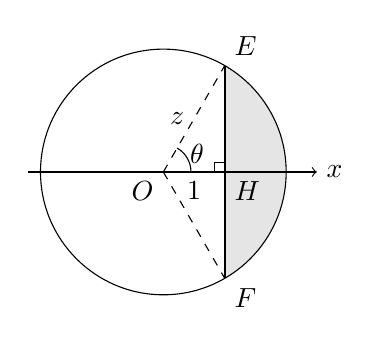
\begin{tikzpicture}[scale=0.78]
                 \fill[gray!20] (1,{-sqrt(3)}) arc[start angle=-60,end angle=60,radius=2] -- cycle;
                 \draw (0,0) circle[radius=2];
                 \draw[thick] (1,{-sqrt(3)}) -- (1,{sqrt(3)});
                 \draw[dashed] (0,0) -- (1,{sqrt(3)}) node[midway,left] {$z$};
                 \draw[dashed] (0,0) -- (1,{-sqrt(3)});
                 \draw[->] (-2.2,0) -- (2.5,0) node[right] {$x$};
                 \draw (0.45,0) arc[start angle=0,end angle=60,radius=0.45];
                 \node at (0.55,0.30) {$\theta$};
                 \node[below left] at (0,0) {$O$};
                 \node[below right] at (1,0) {$H$};
                 \node[above right] at (1,{sqrt(3)}) {$E$};
                 \node[below right] at (1,{-sqrt(3)}) {$F$};
                 \node[below] at (0.5,0) {$1$};
                 \draw (0.84,0) -- (0.84,0.16) -- (1,0.16);
                \end{tikzpicture}
      \BookFigureCaption{立体の水平断面と円弧・弦}
                \end{center}
                その面積を$A(z)$とすると,扇形から三角形を引いて,
                \[
                 \begin{aligned}
                 A(z)&=\frac12z^2\cdot2\theta
                      -\frac12\cdot2\sqrt{z^2-1}\cdot1\\
                     &=z^2\theta-\sqrt{z^2-1}.
                 \end{aligned}
                \]
                よって体積は$V=\int_1^2 A(z)\,dz$である.
                \,$\displaystyle z=\frac{1}{\cos\theta}$と置けば,
                \[
                 \sqrt{z^2-1}=\tan\theta,
                 \qquad dz=\frac{\sin\theta}{\cos^2\theta}\,d\theta.
                \]
                したがって,
                \[
                 \begin{aligned}
                 V&=\int_0^{\frac{\pi}{3}}\frac{\theta\sin\theta}{\cos^4\theta}\,d\theta\\
                  &\quad-\int_0^{\frac{\pi}{3}}\frac{\sin^2\theta}{\cos^3\theta}\,d\theta.
                 \end{aligned}
                \]
                第一項では$\displaystyle (\cos^{-3}\theta)'=\frac{3\sin\theta}{\cos^4\theta}$を使って部分積分する.
                第二項では$\sin^2\theta=1-\cos^2\theta$を使うと,
                \[
                 \begin{aligned}
                 V&=\left[\frac{\theta}{3\cos^3\theta}\right]_0^{\frac{\pi}{3}}
                      -\frac13I_3-(I_3-I_1)\\
                  &=\frac{8\pi}{9}-\frac43I_3+I_1\\
                  &=\frac{8\pi}{9}-\frac{4\sqrt3}{3}
                      +\frac13\log(2+\sqrt3).
                 \end{aligned}
                \]
                断面の半径と切断位置の関係を角度で表すと,最初に調べた$I_3$が自然に現れた.
                積分の\bookterm{recurrence}{漸化式}は\bookterm{sequence}{数列}だけの技法ではなく,図形から生まれる積分を計算するためにも使える.
          % F6: 一般項を求めずに減衰の速さを決める
          \item 分母に$a_n$があるが,本編の分数型と違って分母が二乗になっている.
                まず逆数を取って,\bookterm{general}{一般項}が求められるかだけでなく,増え方を評価できるかを調べる.
                \par\noindent
                \textbf{(1) 逆数の\bookterm{difference}{階差}を足す.}
                $a_1=1>0$であり,$a_n>0$なら$(1+2a_n)^2>0$なので$a_{n+1}>0$である.
                よって\bookterm{induction}{数学的帰納法}からすべての項が正で,$\displaystyle b_n=\frac{1}{a_n}$も定義できる.
                逆数を取ると,
                \[
                 \begin{aligned}
                 b_{n+1}&=\frac{(1+2a_n)^2}{a_n}\\
                         &=b_n+4+4a_n.
                 \end{aligned}
                \]
                したがって$b_{n+1}-b_n=4+4a_n>4$である.
                \,$k=1,\ldots,n-1$について足すと,
                \[
                 b_n-b_1=4(n-1)+4\sum_{k=1}^{n-1}a_k.
                \]
                $b_1=1$より,
                \[
                 b_n=4n-3+4\sum_{k=1}^{n-1}a_k.
                \]
                $n\geq2$なら右辺の総和は正だから,$b_n>4n-3$となる.
                ここまでの変形は,逆数化したあとに\bookterm{difference}{階差}を総和する本編の技法である.
                ただし総和に$a_k$が残っているため,この式だけでは\bookterm{general}{一般項}は得られていない.
                \par\noindent
                \textbf{(2) 項の収束と平均.}
                正の数の逆数を取ると不等号が逆向きになるので,
                \[
                 0<a_n<\frac1{4n-3}\qquad(n\geq2).
                \]
                挟み撃ちの原理より$a_n\to0$である.
                しかし平均にも$n$が入っているので,項の\bookterm{limit}{極限}だけで終えず,平均を直接評価する.
                任意の正数$\varepsilon$を取る.
                \,$a_n\to0$より,$k\geq N$なら$0<a_k<\varepsilon$となる正整数$N$が存在する.
                \,$C=\sum_{k=1}^{N-1}a_k$と置けば,$C$は$n$によらない定数である.
                \,$n\geq N$のとき,
                \[
                 \begin{aligned}
                 0<\frac1n\sum_{k=1}^{n}a_k
                 &=\frac Cn+\frac1n\sum_{k=N}^{n}a_k\\
                 &\leq\frac Cn+\frac{n-N+1}{n}\varepsilon\\
                 &\leq\frac Cn+\varepsilon.
                 \end{aligned}
                \]
                十分大きい$n$では$\displaystyle \frac{C}{n}<\varepsilon$でもあるため,平均は$2\varepsilon$より小さい.
                \,$\varepsilon$はいくらでも小さく取れるので,
                \[
                 \lim_{n\to\infty}\frac1n\sum_{k=1}^{n}a_k=0.
                \]
                この証明では,大きかった最初の有限個の項の影響は$n$で割ると消え,
                残りの項はすべて小さい,という二つの点を使っている.
                \par\noindent
                \textbf{(3) 逆数から減り方を読む.}
                (1)の等式を$n$で割ると,
                \[
                 \frac{b_n}{n}=4-\frac3n+
                            \frac4n\sum_{k=1}^{n-1}a_k.
                \]
                (2)より,
                \[
                 0\leq\frac1n\sum_{k=1}^{n-1}a_k
                 \leq\frac1n\sum_{k=1}^{n}a_k\longrightarrow0.
                \]
                したがって$\displaystyle \frac{b_n}{n}\to4$であり,
                \[
                 na_n=\cfrac{1}{\frac{b_n}{n}}\longrightarrow\frac14.
                \]
                \par
                最初に求めた上界は,$a_n\to0$を示すための中間結果である.
                それによって\bookterm{difference}{階差}の追加項$4a_n$の平均が消え,$b_n$は最終的に$4n$と同じ割合で増えると分かった.
                結論$\displaystyle na_n\to\frac{1}{4}$は,$a_n$の減少の速さが$\displaystyle \frac{1}{4n}$のそれに近づくことを表す.
                このように,\bookterm{general}{一般項}を閉じた式で表さなくても,\bookterm{recurrence}{漸化式}から\bookterm{sequence}{数列}の主要な性質を決められる.
          % F7: 1往復で整列できる札の配置
          \item \textbf{(1)~小さい例と左端の札.}
                  二枚ならすべて成功して$c_2=2$となる.
                  三枚では往路で$3$が右端へ移り,復路の最後に残り二枚が昇順になるので$c_3=6$である.
                  一般に最初の比較後,左端には$b=\min(A_1,A_2)$が残る.
                  その後でこの札に触れるのは復路の最後だけだから,最終位置は左から一番目か二番目である.
                  成功配置では$b\le2$が必要だが,これだけでは十分でない.
                  \smallskip\textbf{(2)~札を戻せる対応.}
                  数字を小さい順に読み替えても,比較・交換の動きは変わらない.
                  (1)により成功配置を次の四種類に分ける.
                  \[
                  \begin{array}{ll}
                    \text{\textcircled{1}}&A_1=1,\\
                    \text{\textcircled{2}}&A_2=1,\\
                    \text{\textcircled{3}}&A_1=2,\ A_2\ge3,\\
                    \text{\textcircled{4}}&A_2=2,\ A_1\ge3.
                  \end{array}
                  \]
                  \textbf{\textcircled{1},\textcircled{2}の数え方.}
                  最初の比較後に左端にある$1$を除くと,残る$n-1$枚への操作は小さい問題と同じになる.
                  復路の最後の$1$との比較は交換を起こさないので,成否も一致する.
                  逆に数字をすべて$1$増やし,$1$を先頭または二番目へ挿入すれば一意に戻せる.
                  よって各種類は$c_{n-1}$通りである.
                  \par\textbf{\textcircled{3}の数え方.}
                  先頭の$2$を除き,$1$はそのまま,$3,\ldots,n$を$2,\ldots,n-1$に読み替える.
                  縮約先の先頭は$1$でない.
                  例えば$(2,4,3,1)$は$(3,2,1)$に対応し,操作は次のようになる.
                  \[
                  \begin{array}{c|c|c}
                    &\text{元の配置}&\text{縮約配置}\\ \hline
                    \text{開始}&(2,4,3,1)&(3,2,1)\\
                    \text{往路後}&(2,3,1,4)&(2,1,3)\\
                    \text{復路後}&(1,2,3,4)&(1,2,3)
                  \end{array}
                  \]
                  \BookMathLayout{一般にも往路後の元の配列は$(2,B_1,\ldots,B_{n-1})$で,後ろの札への操作は縮約問題と同じである.}{一般にも往路後の元の配列は\newline
                  $(2,B_1,\ldots,B_{n-1})$で,後ろの札への操作は縮約問題と同じである.}
                  復路では最小の札$1$がその部分の左端へ移るため,最後の比較直前には
                  $(2,1,D_2,\ldots,D_{n-1})$となる.
                  最後の$(2,1)$を交換すれば,元の成否と縮約先の成否が一致する.
                  逆に,先頭が$1$でない成功配置で数字$2$以上を$1$増やし,先頭に$2$を戻せば一意に復元できる.
                  先頭が$1$の成功配置は\textcircled{1}の対応から$c_{n-2}$通りなので,
                  \textcircled{3}は$c_{n-1}-c_{n-2}$通りとなる.
                  \par\textbf{\textcircled{4}の数え方.}
                  最初の二枚を交換すれば\textcircled{3}に一対一で対応し,最初の比較後は同じ配列になる.
                  よってこちらも$c_{n-1}-c_{n-2}$通りであり,
                  \[
                    c_n=2c_{n-1}+2(c_{n-1}-c_{n-2})
                       =4c_{n-1}-2c_{n-2}.
                  \]
                  引いた$c_{n-2}$は,\textcircled{3}の縮約先から除く「先頭が$1$の配置」の数である.
                  \smallskip\textbf{(3)~個数から3項型へ.}
                  \bookterm{characteristic}{特性方程式}$x^2-4x+2=0$の根は$2\pm\sqrt2$である.
                  \[
                    c_n=P(2+\sqrt2)^{n-1}+Q(2-\sqrt2)^{n-1}
                  \]
                  に$c_1=1,c_2=2$を入れると$P=Q=\dfrac{1}{2}$であり,解答の式を得る.
                  $c_4=20,c_5=68$となる.二つのべきで$\sqrt2$の奇数次の項が相殺され,個数は整数になる.
                  この問の中心は,解く前の「何を取り除き,どう戻すか」という設計にある.
          % F8: 巨大な項の整除と, 添字の互除法
          \item \textbf{(1)~余りの\bookterm{recurrence}{漸化式}.}\par\nobreak
                  項は$1,2,5,26,677,\ldots$と急増するが,法$5$で余りの更新を追えば,
                  \[
                    1\longmapsto2\longmapsto0\longmapsto1
                  \]
                  と繰り返す.同じ余りから次は一意に決まるため,$5$の倍数となるのは$n=3,6,9,\ldots$である.
                  \smallskip\textbf{(2)~項を法に取る.}
                  $a_0=0$を補えば更新は$n\ge0$で使える.正整数$m$を固定すると,
                  \[
                    a_{m+j}\equiv a_j\pmod{a_m}\quad(j\ge0)
                  \]
                  が成り立つ.$j=0$では両辺が零であり,次も$a_{m+j}^2+1\equiv a_j^2+1$なので,
                  \bookterm{induction}{数学的帰納法}で示せる.
                  $n=qm+r$（$0\le r<m$）としてこの合同式を繰り返すと,
                  $a_n\equiv a_r\pmod{a_m}$となる.
                  また$a_{n+1}-a_n=a_n(a_n-1)+1>0$より$a_0$から厳密に増加するので,
                  $0\le a_r<a_m$かつ$a_r=0$は$r=0$の場合だけである.
                  よって,
                  \[
                    \begin{aligned}
                    a_m\mid a_n&\ \Longleftrightarrow\ a_r=0\\
                      &\ \Longleftrightarrow\ r=0\ \Longleftrightarrow\ m\mid n.
                    \end{aligned}
                  \]
                  $m=1$でも$r=0$なので成り立つ.(1)は$a_3=5$を用いた$m=3$の場合に当たる.
                  \smallskip\textbf{(3)~項から添字の互除法へ.}
                  $a_n-a_r$は$a_m$の倍数なので,共通の約数は変わらず,
                  \[
                    \gcd(a_m,a_n)=\gcd(a_m,a_r).
                  \]
                  \BookMathLayout{添字の互除法に沿って進むと,$d=\gcd(m,n)$と$0$で終わるため,}{添字の互除法に沿って進むと,\newline
                  $d=\gcd(m,n)$と$0$で終わるため,}
                  \[
                    \gcd(a_m,a_n)=\gcd(a_d,a_0)=a_d.
                  \]
                  最後は$a_0=0$と$\gcd(x,0)=x$を使った.
                  例では$3040=2026+1014$, $2026=1014+1012$, $1014=1012+2$, $1012=506\cdot2$より$d=2$である.
                  したがって$\gcd(a_{2026},a_{3040})=a_2=2$となる.
                  巨大な項どうしの整除関係を,小さな添字の計算へ移せた.
          % F9: 整数方程式の解を生み出す漸化式
          \item \textbf{(1)~一つの解から次の解へ.}
                  $9+y^2+z^2=3yz$を$y$の二次方程式と見ると,もう一つの根は$3z-y$である.
                  実際,
                  \[
                    \begin{aligned}
                    &9+z^2+(3z-y)^2-3z(3z-y)\\
                    &\qquad=9+y^2+z^2-3yz=0.
                    \end{aligned}
                  \]
                  $3z-y$は整数で,$0<y\le z$より$3z-y\ge2z>z>0$となる.
                  新しい二項も大小関係を満たすため,操作を繰り返せる.
                  \smallskip\textbf{(2)~整数解を\bookterm{sequence}{数列}にする.}
                  $(3,3,3)$からの操作で,$y,z$は$(3,3),(3,6),(6,15),(15,39),\ldots$と変わる.
                  隣接する値を$u_n,u_{n+1}$とすれば$u_{n+2}=3u_{n+1}-u_n$となる.
                  \bookterm{characteristic}{特性方程式}$t^2-3t+1=0$の根を$\alpha,\beta$とし,
                  $u_n=P\alpha^n+Q\beta^n$とおく.
                  $u_0=u_1=3$から,
                  \[
                    P=\frac{3(\sqrt5-1)}{2\sqrt5},\quad
                    Q=\frac{3(\sqrt5+1)}{2\sqrt5}
                  \]
                  となり,解答の式を得る.
                  \smallskip\textbf{(3)~整数性と方程式の確認.}
                  初期値と更新の係数から全項が整数である.
                  $u_2=6>u_1=3$であり,$u_{n+1}>u_n>0$なら$u_{n+2}>2u_{n+1}>u_{n+1}$となるため,
                  $n\ge1$で正値と厳密な増加が続く.
                  隣接する二項から作る
                  \[
                    I_n=u_n^2+u_{n+1}^2-3u_nu_{n+1}
                  \]
                  に更新式を入れると,
                  \[
                  \begin{aligned}
                    I_{n+1}&=u_{n+1}^2+(3u_{n+1}-u_n)^2\\
                           &\quad-3u_{n+1}(3u_{n+1}-u_n)=I_n.
                  \end{aligned}
                  \]
                  よって$I_n=I_0=-9$から$(3,u_n,u_{n+1})$は正の整数解となる.
                  増加するため解は互いに異なり,無限個得られる.ここでは全解の分類まではしていない.
                  最後に$0<\beta<1<\alpha$と$P,Q>0$から,
                  \[
                    \frac{u_{n+1}}{u_n}
                      =\alpha\,\cfrac{P+Q(\frac\beta\alpha)^{n+1}}
                                       {P+Q(\frac\beta\alpha)^n}
                      \longrightarrow\alpha.
                  \]
                  更新式は整数性を保証し,\bookterm{general}{一般項}は整数の比が近づく無理数を示している.
          % F10: 元のペアをすべて解消する組み替え
          \item \textbf{(1) 小さい場合を数える.}
                  $n=1$では相手がいないので$S(1)=0$である.
                  $n=2$では$(A_1,B_2),(A_2,B_1)$の一通り,
                  $n=3$では相手の添字が$(2,3,1),(3,1,2)$の二通りである.
                  $S(0)=1$は「何も作らない組合せ」を一通りと数える約束である.
                  \par\smallskip\textbf{(2) 相手を決めて分ける.}
                  $A_1$の相手$B_j$を$j\ne1$の$n-1$通りから選び,固定する.
                  $A_j$の相手が$B_1$なら,この二組の四要素を除く.
                  残る添字は両側とも$1,j$以外であり,同じ添字のペアを禁止する条件も変わらない.
                  したがって,残る$n-2$組の組み方は$S(n-2)$通りである.
                  そうでない場合,$B_1$の相手を$A_k$（$k\ne1,j$）とする.
                  この場合に四要素をそのまま除くと,両側で消える添字が異なり,残る問題の条件が変わってしまう.
                  そこで,二組を一組につなぎ直す.
                  \[
                    (A_1,B_j),(A_k,B_1)\ \longmapsto\ (A_k,B_j)
                  \]
                  除くのは$A_1,B_1$だけで,$A_k,B_j$は残る.
                  $k\ne j$なので新しいペアも元のペアではなく,ほかのペアは変わらない.
                  これで,添字$2,\ldots,n$の元のペアを一組も含まない組み替えが得られる.
                  \par
                  逆に,この$n-1$組の組み替えを任意に取る.
                  $B_j$の相手は一意に決まる$A_k$であり,元のペアがないので$k\ne j$である.
                  $(A_k,B_j)$を$(A_1,B_j),(A_k,B_1)$に戻せば,元の配置を一意に復元できる.
                  この一対一対応から,後者は$S(n-1)$通りである.
                  ここで固定しているのは$j$であり,$k$の異なる場合はすべて$S(n-1)$に含まれている.
                  $j$の選び方が$n-1$通りなので,
                  \[
                    S(n)=(n-1)\{S(n-1)+S(n-2)\}.
                  \]
                  \par\smallskip\textbf{(3) 差と階乗で整理する.}
                  係数が$n$で変わるため,\bookterm{constant}{定数係数}の特性方程式は使えない.
                  $T_n=S(n)-nS(n-1)$とおくと,$n\ge2$で,
                  \[
                    T_n=(n-1)S(n-2)-S(n-1)=-T_{n-1}.
                  \]
                  $T_1=-1$から$T_n=(-1)^n$となる.
                  $S(n)=nS(n-1)+(-1)^n$の両辺を$n!$で割り,$P_n=\dfrac{S(n)}{n!}$とおけば,
                  \[
                    P_n-P_{n-1}=\frac{(-1)^n}{n!},\quad P_0=1.
                  \]
                  \bookterm{difference}{階差}を足すと,
                  \[
                    S(n)=n!\sum_{k=0}^n\frac{(-1)^k}{k!}.
                  \]
                  $S(4)=9,S(5)=44$となる.
                  等比型,\bookterm{ratio}{階比}による\bookterm{normalize}{正規化},\bookterm{difference}{階差}型を順に使った.
                  \par\smallskip\textbf{(4) 残る組数で数える.}
                  残す$r$組を選び,残りを完全に組み替えれば$\binom nrS(n-r)$通りである.
                  残るペアは完成形から一意に決まり,$r=n$も$S(0)=1$によって含む.
                  平均には,固定した元のペアが残る$(n-1)!$通りを$n$組分数える.
                  $r$組残る配置は$r$回数えられるので,残る組数の合計は$n(n-1)!$であり,平均は$\dfrac{n(n-1)!}{n!}=1$となる.
                  \par\smallskip\noindent\textbf{【確率として読む】}\par\nopagebreak[4]
                  元の位置に戻る要素のない並べ替えを\textbf{完全順列（錯置）}という.
                  全$n!$通りが等確率なら,元のペアが一組も残らない確率は,
                  \[
                    P_n=\frac{S(n)}{n!}=\sum_{k=0}^n\frac{(-1)^k}{k!}.
                  \]
                  階乗で割る操作は,\textbf{個数を確率に直す操作}でもある.
                  \par\smallskip\noindent\textbf{【偶奇に分けて極限を確かめる】}\par\nopagebreak[4]
                  まず収束を示し,その後で値を決める.無限級数展開は仮定せず,
                  \bookterm{binomial}{二項定理}と\sectionref*{節：対数}の$e$の定義を使う.
                  \[
                  \begin{aligned}
                    P_{2m+2}-P_{2m}&=-\frac{2m+1}{(2m+2)!}<0,\\
                    P_{2m+3}-P_{2m+1}&=\frac{2m+2}{(2m+3)!}>0,\\
                    P_{2m}-P_{2m+1}&=\frac1{(2m+1)!}\longrightarrow0.
                  \end{aligned}
                  \]
                  偶数番目は減少,奇数番目は増加し,確率は$0$以上$1$以下である.
                  よって両者は共通の\bookterm{limit}{極限}$L$をもつ.
                  \par\smallskip\noindent\textbf{【二項定理で極限の値を決める】}\par\nopagebreak[4]
                  整数$M\ge2$について$b_{M,k}=\dfrac{\binom Mk}{M^k}$とおくと,
                  \[
                    \frac{b_{M,k+1}}{b_{M,k}}=\frac{M-k}{M(k+1)}\le1
                    \quad(0\le k<M).
                  \]
                  有限の二項展開を途中で止め,残りを隣り合う二項ずつ組にする.
                  奇数で止めた残りは非負,偶数で止めた残りは非正なので,$M\ge2\ell+1$では,
                  \[
                  \begin{aligned}
                    \sum_{k=0}^{2\ell+1}(-1)^kb_{M,k}
                      &\le\left(1-\frac1M\right)^M,\\
                    \left(1-\frac1M\right)^M
                      &\le\sum_{k=0}^{2\ell}(-1)^kb_{M,k}.
                  \end{aligned}
                  \]
                  \textbf{まず$\ell$を固定して$M\to\infty$とする.}
                  和の項数は固定され,各項で,
                  \[
                    b_{M,k}=\frac1{k!}\prod_{j=0}^{k-1}\left(1-\frac jM\right)
                      \longrightarrow\frac1{k!}
                  \]
                  となる.$k=0$の空積は$1$である.
                  一方,$t=M-1$とおくと,
                  \[
                    \left(1-\frac1M\right)^M=\left(1+\frac1t\right)^{-t-1}
                      \longrightarrow\frac1e
                  \]
                  である.$\left(1+\dfrac{1}{t}\right)^t\to e$と$1+\dfrac{1}{t}\to1$を使った.
                  したがって$P_{2\ell+1}\le\dfrac{1}{e}\le P_{2\ell}$となる.
                  \textbf{次に$\ell\to\infty$とする.}両端が$L$へ近づくため,
                  \[
                    \boxed{\lim_{n\to\infty}\frac{S(n)}{n!}=\frac1e\simeq0.368}.
                  \]
                  \par\smallskip\noindent\textbf{【個数はどこまで近いか】}\par\nopagebreak[4]
                  偶奇の各列が厳密に進むので,$\dfrac{1}{e}$は隣り合う$P_n,P_{n+1}$の間に厳密に入る.
                  よって$n\ge1$で,
                  \[
                  \begin{aligned}
                    \left|P_n-\frac1e\right|&<\frac1{(n+1)!},\\
                    \left|S(n)-\frac{n!}e\right|&<\frac1{n+1}\le\frac12.
                  \end{aligned}
                  \]
                  下段は上段を$n!$倍したものであり,$S(n)$は$\dfrac{n!}{e}$に最も近い整数となる.
                  数え上げの\bookterm{recurrence}{漸化式}が,階乗・確率・自然\bookterm{logarithm}{対数}の底を結んだ.
        \end{enumerate}
